% !TEX root = main.tex
\chapter[head={\CP violation in the $B$-meson sector},tocentry={$\symbfsf{C{}P}$ violation in the $\symbfsf{B}$-meson sector}]
{$\symbfsf{C{}P}$ violation in the $\symbfsf{B}$-meson sector}
\label{chap:CPV}

Since $CPT$ is conserved in the \ac{SM} the violation of \CP is equivalent to a violation of the $T$ symmetry.
As described in \cref{sec:symmetriesInSM} the $T$ operator is antiunitary and therefore it transforms numbers into their complex conjugate.
Hence the \CP transformation also affects only the complex phases of the bras and kets describing initial and final states.
However the absolute values of phases describing transitions between different states are not physically meaningful as the bras and kets can be rephased at will.
The physical meaningful quantities are the relative phase differences between coherent contributions to a transition, as these are invariant under global rephasings.
There are three types of phases arising in transition amplitudes:
\emph{Weak} phases, which change sign under \CP transformation (\CP-odd), \emph{strong} phases, which do not change sign under \CP transformation (\CP-even) and \emph{spurious} phases, which usually arise due to conventional rephasings.
The denotations \emph{weak} and \emph{strong} do not mean that the phases originate in weak or strong interactions, but only describe their behaviour under \CP transformation.
Spurious phases are global and just arise due to conventional rephasings.
As they do not originate in any dynamics they will be ignored below for simplification.
Consequently the \CP transformation of the initial and final states are defined with \emph{weak} phases $\xi_i$ and $\xi_f$ as follows
\begin{equation}
\begin{aligned}
&\CP\left|\Bz\right> =e^{i\xi}\left|\Bzb\right>&&\CP\left|\Bzb\right>=e^{-i\xi}\left|\Bz\right>&\\
&\CP\left|\,\f\,\right> =e^{i\xi_f}\left|\,\fbar\,\right>&&\CP\left|\,\fbar\,\right>=e^{-i\xi_f}\left|\,\f\,\right>.& \label{eq:CPTransInitFinal}
\end{aligned}
\end{equation}

In this chapter first the time evolution of neutral mesons by example of uncharged \B-mesons is described and then the three classes of \CP violation are discussed. More details on these topics can be found in Refs.~\cite{Branco:396964,Bigi:1295518}

\section[head={Time evolution of neutral \B-mesons},tocentry={Time evolution of neutral \B-mesons}]{Time evolution of neutral $\symbfsf{\B}$-mesons}
\label{sec:TimeEvolution}

As previously described in \cref{sec:unitarityTriangle} for the quarks the mass eigenstates and the eigenstates of the weak interaction are not identical.
The same applies for bound states of quarks like \B-mesons. Studying the system of a \Bz (\bquarkbar\dquark) and a \Bzb-meson
(\bquark\dquarkbar), the most general description to determine the time evolution is the Schrödinger equation:
\begin{equation}
i\frac{d}{dt}\begin{pmatrix} \Bz \\ \Bzb \end{pmatrix} = H \begin{pmatrix} \Bz \\ \Bzb \end{pmatrix}
=\left(M-\frac{i}{2}\Gamma\right)\begin{pmatrix} \Bz \\ \Bzb \end{pmatrix}, \label{eq:mixMatrix}
\end{equation}
with $M$ and $H$ being 2x2 hermitian 2x2 matrices.
Hence, the matrix $H$ is not hermitian and allows the \B mesons to decay and not just to oscillate.
In possible transitions virtual intermediate states contribute to the matrix $M$ while real physical states to which \Bz and \Bzb decay contribute to the matrix $\Gamma$.
Furthermore, as due to the $CPT$ theorem particle and antiparticles have the same masses and decay widths the following constraints apply for the matrix elements:
\begin{equation}
\begin{aligned}
&m_{11}=m_{22}\equiv m&&m_{12}=m_{21}^\ast&\\
&\Gamma_{11}=\Gamma_{22}\equiv\Gamma&&\Gamma_{12}=\Gamma_{21}^\ast&
\end{aligned}
\end{equation}
Interpreting \Bz and \Bzb as two states distinguished by an internal quantum number $F$ the matrix elements can also be classified by certain types of transitions:
transitions with $\Delta F=1$ are driven by the diagonal elements, while the off diagonal elements are describe with $\Delta F=2$.
These $\Delta F=2$ processes describe so-called particle-antiparticle-oscillations.
The Feynman graphs of lowest order for these oscillations are shown in \cref{fig:FeynmanMixing}.
\begin{figure}[tbp]
	\centering
	\includestandalone{03CPV/figs/Bmixing_1}
	\hspace{0.5cm}
	\includestandalone{03CPV/figs/Bmixing_2}
	\caption{Box diagrams of lowest order for the \Bz-\Bzb-oscillation. Both diagrams are dominated by the \tquark-quark \cite{Ellis:2016jkw}.}
	\label{fig:FeynmanMixing}
\end{figure}

To solve \cref{eq:mixMatrix} and infer the time evolution the matrix $H$ needs to be diagonalised to obtain the mass eigenstates and the corresponding eigenvalues.
In the \Bz-meson system the mass eigenstates are denoted with $\B_H$ and $\B_L$ referring to the heavier and lighter eigenstate, respectively.
Using
\begin{equation}
F=\sqrt{\left(m_{12}-\frac{i}{2}\Gamma_{12}\right)\left(m_{12}^\ast-\frac{i}{2}\Gamma_{12}^\ast\right)}.
\end{equation}
the eigenvalues can be expressed as
\begin{equation}
\begin{split}
\mu_H &= m_H-\frac{i}{2}\GH = m + \mathcal{Re}\left(F\right)-\frac{i}{2}\left(\Gamma-2\mathcal{Im}\left(F\right)\right)\\
\mu_L &= m_L-\frac{i}{2}\GL = m - \mathcal{Re}\left(F\right)-\frac{i}{2}\left(\Gamma+2\mathcal{Im}\left(F\right)\right)\label{eq:Mass_eigenvalues}
\end{split}
\end{equation}
with the eigenstates
\begin{equation}
\begin{split}
\left|B_H\right>&= p\left|\Bz\right>+q\left|\Bzb\right>\\
\left|B_L\right>&= p\left|\Bz\right>-q\left|\Bzb\right>.\label{eq:Mass_eigenstates}
\end{split}
\end{equation}
The parameters $p$ and $q$ are constrained to fulfil $\left|p\right|^2+\left|q\right|^2=1$ by construction and their ratio $\frac{q}{p}$ can be expressed in terms of the matrix elements:
\begin{equation}
\frac{q}{p}=\sqrt{ \frac{ m_{12}^\ast-\frac{i}{2}\Gamma_{12}^\ast }{ m_{12}-\frac{i}{2}\Gamma_{12} }}
=\frac{\dm-\frac{i}{2}\DG}{2\left(m_{12}-\frac{i}{2}\Gamma_{12}\right)}.\label{eq:qoverp}
\end{equation}
Using the mass eigenvalues from \cref{eq:Mass_eigenvalues} and mass eigenstates from \cref{eq:Mass_eigenstates} and the Schrödinger equation can be rewritten as
\begin{equation}
i\frac{d}{dt}\begin{pmatrix} B_L \\ B_H \end{pmatrix} = \begin{pmatrix} \mu_L & 0 \\ 0 & \mu_H \end{pmatrix}\begin{pmatrix} B_L \\ B_H \end{pmatrix},
\end{equation}
which can be easily solved and leads to the time evolution of the mass eigenstates with simple exponential functions $B_{L,H}=e^{-i\mu_{L,H}t}B_{L,H}$.
Inverting \cref{eq:Mass_eigenstates} the time evolution for the flavour eigenstates follows straightforward:
\begin{equation}
\begin{split}
\left|\Bz\!\left(t\right)\right>&=\left|\Bz\right>g_+-\frac{q}{p}\left|\Bzb\right>g_-\\
\left|\Bzb\!\left(t\right)\right>&=\left|\Bzb\right>g_--\frac{p}{q}\left|\Bz\right>g_+ \label{eq:timeEvolution}
\end{split}
\end{equation}
with $g_\pm=\frac{1}{2}\left(e^{-i\mu_Ht}\pm e^{-i\mu_Lt}\right)$.
The associated masses and decay widths of the eigenstates of the weak interaction can be written as
\begin{equation}
m=\frac{m_L+m_H}{2}\hspace{0.5cm}\text{and}\hspace{0.5cm}\Gamma=\frac{\GL+\GH}{2}.
\end{equation}
The corresponding differences will be referred to as
\begin{equation}
\dm=m_H-m_L=2\mathcal{Re}\left(F\right)\hspace{0.5cm}\text{and}\hspace{0.5cm}\DG=\GL-\GH=4\mathcal{Im}\left(F\right).
\end{equation}

\section[head={Classes of \CP violation},tocentry={Classes of \CP violation}]{Classes of $\symbfsf{C{}P}$ violation}
\label{sec:CPVClasses}

Depending on the type of transition in which \CP violation occurs, its manifestation is different, yielding in three classes.
Transitions with purely $\Delta F=1$ are affected by the so-called direct \CP violation, in transitions with $\Delta F=2$ \CP violation in mixing can potentially be observed.
Transitions affected by both $\Delta F=1$ dynamics and $\Delta F=2$ dynamics can be additionally affected by the so-called interference \CP violation.
Using the following notation for the decay amplitudes
\begin{equation}
\begin{split}
\Af = \left<\,f\,\Big|T\Big|\Bz\right>\hspace{1cm}\Afbar = \left<\,\fbar\,\Big|T\Big|\Bz\right>\\
\Abarf = \left<\,f\,\Big|T\Big|\Bzb\right>\hspace{1cm}\Abarfbar = \left<\,\fbar\,\Big|T\Big|\Bzb\right>
\end{split}
\end{equation}
these three types will be described in more detail below.


\subsection[head={Direct \CP violation},tocentry={Direct \CP violation}]{Direct $\symbfsf{C{}P}$ violation}
\label{sec:DirectCPV}

Direct \CP violation or \CP violation in decay means that a specific decay amplitude differs between the particle and its corresponding antiparticle.
It is the only type of \CP violation which can occur for charged particles.
Experimentally this can be measured with a \CP asymmetry like
\begin{equation}
A_{\CP}=\frac{\left|\left<\,\fbar\,|T|\,\Bzb\,\right>\right|^2-\left|\left<\,\f\,|T|\,\Bz\,\right>\right|^2}{\left|\left<\,\fbar\,|T|\,\Bzb\,\right>\right|^2+\left|\left<\,\f\,|T|\,\Bz\,\right>\right|^2} = \frac{\left|\,\nicefrac{\Abarfbar}{\Af}\,\right|^2-1}{\left|\,\nicefrac{\Abarfbar}{\Af}\,\right|^2+1}.
\end{equation}
Naively one could expect that it is sufficient that a single amplitude contributes to a transition.
But considering a decay with just one amplitude
\begin{equation}
\begin{split}
\Af&=Ae^{i\left(\delta+\phi\right)}\\
\Abarfbar&=Ae^{i\left(\delta-\phi\right)}
\end{split}
\end{equation}
where $A$ is a real positive number, $\phi$ is the \emph{weak} phase and $\delta$ the \emph{strong} phase, it becomes immediately obvious that the quantity $\big|\,\Abarfbar\,\big|^2-\big|\,\Af\,\big|^2$ vanishes and therefore \CP is conserved.
When instead considering a decay with two contributing amplitudes with different \emph{weak} and \emph{strong} phases
\begin{equation}
\begin{split}
\Af=A_1e^{i\left(\delta_1+\phi_1\right)}+A_2e^{i\left(\delta_2+\phi_2\right)}\\
\Abarfbar=A_1e^{i\left(\delta_1-\phi_1\right)}+A_2e^{i\left(\delta_2-\phi_2\right)}
\end{split}
\end{equation}
\CP violation becomes possible if both the \emph{weak} and the \emph{strong} phases differ:
\begin{equation}
\left|\,\Af\,\right|^2-\left|\,\Abarfbar\,\right|^2=-4A_1A_2\sin\left(\delta_1-\delta_2\right)\sin\left(\phi_1-\phi_2\right).
\end{equation}
For \B-mesons this has been measured by the \lhcb experiment in the decay modes $\Bz\to\Kp\pim$ and $\Bs\to\Km\pip$ \cite{LHCb-PAPER-2013-018} to be
\begin{equation}
\begin{split}
A_{\CP}\left(\Bz\to\Kp\pim\right) &= -0.080\pm0.007\stat \pm 0.003\syst\\
A_{\CP}\left(\Bs\to\Km\pip\right) &= 0.27\pm0.04\stat \pm 0.01\syst
\end{split}
\end{equation}
what corresponds to a statistical significance of $10.5\sigma$ and $6.5\sigma$ for the \Bz and the \Bs mode, respectively.
Figure \ref{fig:DirectCPV} shows the corresponding invariant mass spectra.
\begin{figure}[tbp]
	\centering
	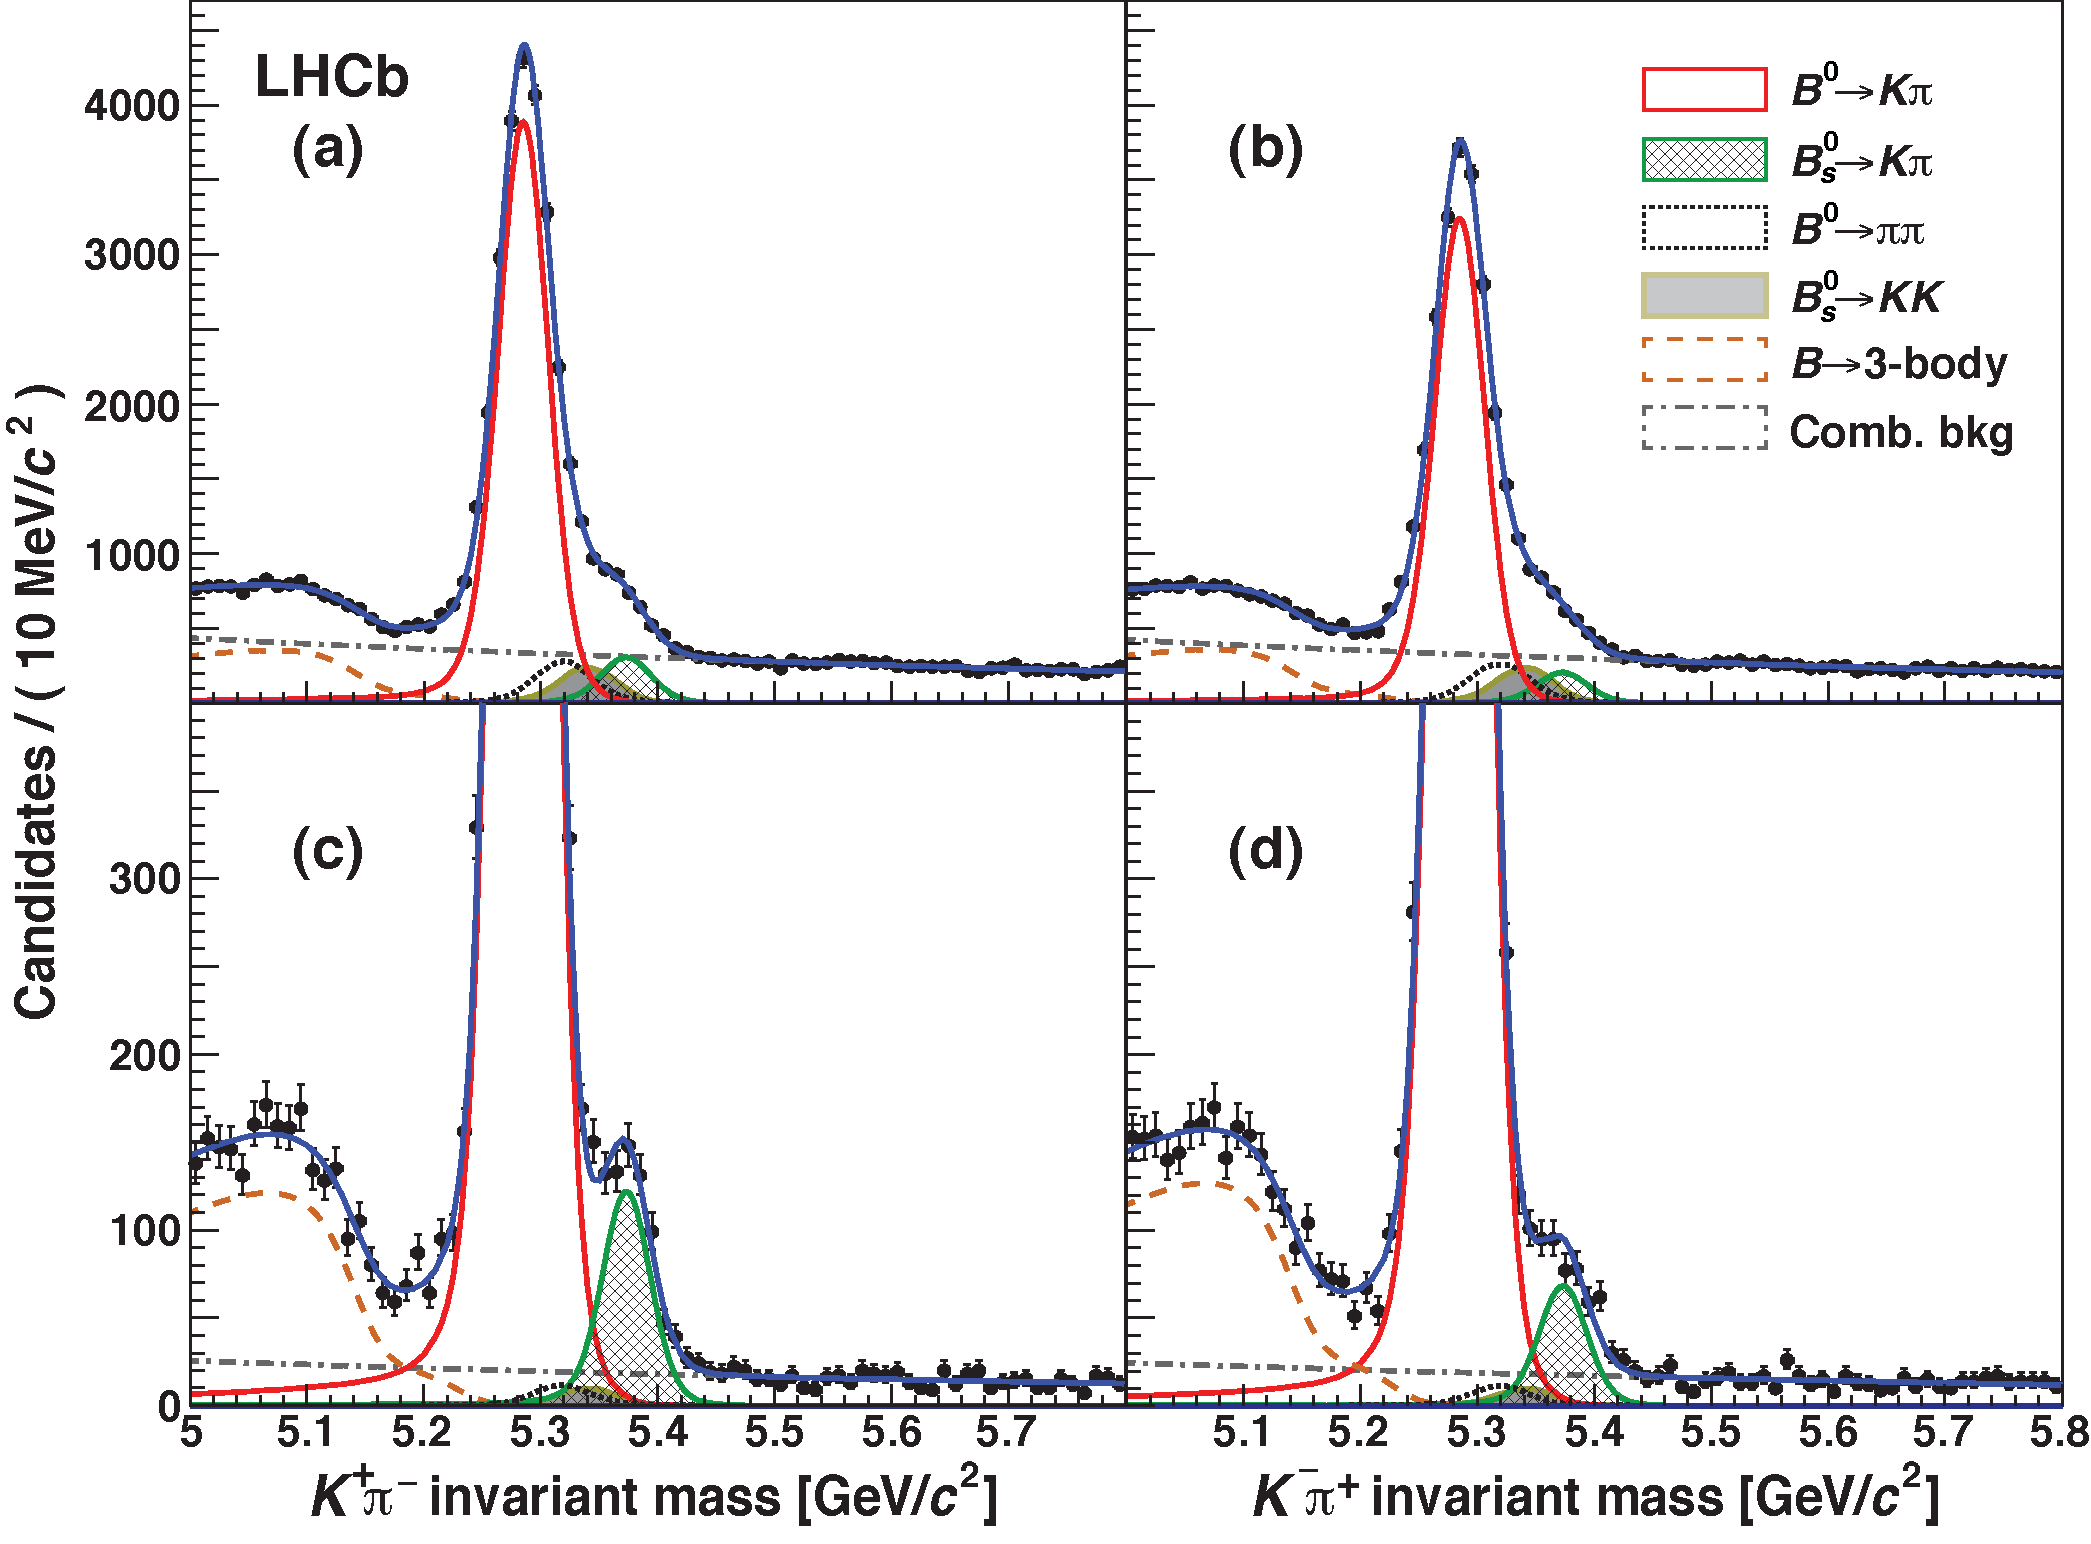
\includegraphics[width=0.8\textwidth]{03CPV/figs/DirectCPV.pdf}
	\caption{Invariant mass spectra obtained with the event selection for the best sensitivity on $A_{\CP}\left(\Bz\to\Kp\pim\right)$ (a,b) and $A_{\CP}\left(\Bs\to\Km\pip\right)$ (c,d). The figures (a) and (c) show the invariant mass distributions for \Kp\pim, figures (b) and (d) show the invariant mass distributions for \Km\pip.}
	\label{fig:DirectCPV}
\end{figure}


\subsection[head={Mixing \CP violation},tocentry={Mixing \CP violation}]{Mixing $\symbfsf{C{}P}$ violation}
\label{sec:MixingCPV}

Indirect \CP violation, also denoted as \CP violation in mixing implies that the transition probabilities for a \Bz-meson to oscilate into a \Bzb meson and vice versa are different.
As due to charge conservation mxing is only possible for uncharged mesons this type of \CP violation cannot occur for charged particles.
Using the time evolution from \cref{eq:timeEvolution} the probabilities of initially produced \Bz and \Bzb mesons to have oscillated within a proper-time $t$ are
\begin{align}
\left|\left<\Bz\Big|\Bzb\!\left(t\right)\right>\right|^2=\frac{1}{4}\left|\frac{p}{q}\right|^2
\left(e^{-\GH t}+e^{-\GL t}-2e^{\frac{1}{2}\left(\Gamma\right)t}\cos\left(\dm t\right)\right),\\
\left|\left<\Bzb\Big|\Bz\!\left(t\right)\right>\right|^2=\frac{1}{4}\left|\frac{q}{p}\right|^2
\left(e^{-\GH t}+e^{-\GL t}-2e^{\frac{1}{2}\left(\Gamma\right)t}\cos\left(\dm t\right)\right).
\end{align}
To obtain the same probabilities for both processes obviously
\begin{equation}
\left|\frac{q}{p}\right|=\left|\frac{p}{q}\right| \Rightarrow \left|\frac{q}{p}\right|=1
\end{equation}
is required.
According to \cref{eq:qoverp} this means that indirect \CP violation occurs if the matrix elements $m_{12}$ and $\Gamma_{12}$ have different complex phases.
The \CP asymmetry in case of indirect \CP violation can be defined as
\begin{equation}
A_{\CP}(t)=\frac{\Gamma\left(\Bz\to\Bzb\right) - \Gamma\left(\Bzb\to\Bz\right)}{\Gamma\left(\Bz\to\Bzb\right) + \Gamma\left(\Bzb\to\Bz\right)}
= \frac{1-\left|\nicefrac{p}{q}\right|^4}{1+\left|\nicefrac{p}{q}\right|^4}
\end{equation}
However, as neutral \B-mesons do not just oscillate but also decay this asymmetry can not be used directly to measure \CP violation in mixing.
Instead the \B-mesons need to be reconstructed in flavour specific decays, \ie only the transitions $\Bz\to\f$ and $\Bzb\to\fbar$, but not $\Bz\to\fbar$ and $\Bzb\to\f$ are allowed.
Thus the flavour of the meson at decay can be determined by final state and compared to the initial production flavour.
For the \Bz and \Bs meson system \CP violation in mixing has been measured to be negligible \cite{HFLAV2016} what is in good agreement with the \ac{SM} predictions.

\subsection[head={Interference \CP violation},tocentry={Interference \CP violation}]{Interference $\symbfsf{C{}P}$ violation}
\label{sec:InterferenceCPV}

So far \CP violation arising due to a clash between the phases of two interfering decay amplitudes or a clash between the phases of $m_{12}$ and $\Gamma_{12}$ has been discussed.
The third possibility is a clash between the phase of $\nicefrac{q}{p}$ and the phase of the decay amplitude what results in the so-called interference \CP violation.
For this class of \CP violation decays of \Bz and \Bzb mesons into both the final state \f and its \CP-conjugate \fbar need to be considered.

Inverting the requirement for \CP violation in mixing shows that \CP is conserved when there is a phase $\xi'$ such that
\begin{equation}
\begin{split}
m_{12}^\ast &= e^{2i\xi'}m_{12}\\
\Gamma_{12}^\ast &= e^{2i\xi'}\Gamma_{12}\label{eq:CPconservationMixing}
\end{split}
\end{equation}
what leads directly to $\nicefrac{q^2}{p^2} = e^{2i\xi'}$.
Using \cref{eq:CPTransInitFinal} the \CP conjugated amplitudes \Abarfbar and \Afbar can be expressed as
\begin{align}
\Abarfbar&=e^{i\left(\xi_f-\xi\right)}\Af,\label{eq:amplitudetransformation_1}\\
\Afbar&=e^{i\left(\xi_f+\xi\right)}\Abarf.\label{eq:amplitudetransformation_2}
\end{align}
what leads to $\big|\,\Af\,\big|=\big|\,\Abarfbar\,\big|$ and $\big|\,\Abarf\,\big|=\big|\,\Afbar\,\big|$ after eliminating the phases and shows that these amplitudes are \CP conserving.
Combining \cref{eq:amplitudetransformation_1} and \cref{eq:amplitudetransformation_2} then leads to
\begin{equation}
\Af\,\Afbar=e^{2i\xi}\,\Abarfbar\,\Abarf\,.
\end{equation}
Under the assumption that the phase of $\nicefrac{q}{p}$ and the phases of the decay amplitudes do not clash, \ie $\xi=\xi'$, \CP is conserved and
\begin{equation}
\arg\left(\frac{p^2}{q^2}\Af \,\overline{\kern -1.0pt A\kern -1.0pt}_{\kern 1.0pt f}^\ast\,\Afbar\overline{\kern -1.0pt \,A\kern -1.0pt}_{\kern 2.5pt\overline{\kern -1.5pt f\kern 1.5pt}}^\ast\right)=0
\end{equation}
applies.
This can be reformulated using the parameters
\begin{equation}
\Lf=\frac{q}{p}\frac{\Abarf}{\Af}\hspace{0.5cm}\text{and}
\hspace{0.5cm}\Lfbar=\frac{p}{q}\frac{\Afbar}{\Abarfbar}.
\end{equation}
Even without \CP violation in decay or mixing ($\big|\Lf\big|=\big|\Lfbar\big| = \pm1$) \CP is not conserved in case of
\begin{equation}
	\arg\left(\Lf\right)-\arg\left(\Lfbar\right)\neq0. \label{eq:conditionCPV}
\end{equation}

This type of \CP violation was first measured by the \B-factories \babar \cite{Aubert:2001nu} and \belle \cite{Abe:2001xe}.
The most prominent measurement is probably the anlysis of the so-called golden mode \BdToJPsiKS to determine $\sin{}\left(2\beta\right)$.
For this decay channel the condition in \cref{eq:conditionCPV} can be simplified to $\arg\left(\Lf\right)\neq0$ as only one common finalstate for both \Bz and \Bzb exists.
Furthermore no \CP violation in decay and mixing is expected for the decay \BdToJPsiKS and with the current experimental precision $\DG=0$ can be assumed.
Therefore the \CP asymmetry can be expressed as
\begin{equation}
A_{\CP}(t)=\frac{\Gamma\left(\Bzb\to\jpsi\KS\right)-\Gamma\left(\BdToJPsiKS\right)}{\Gamma\left(\Bzb\to\jpsi\KS\right)+\Gamma\left(\BdToJPsiKS\right)}=\Sf\sin\left(\dmd t\right),
\end{equation}
with the parameter $\Sf=\sin{}\left(2\beta\right)$ (a more thoroughly description of the formalism will be given in \cref{ch:CKMAngleGamma}).
The most recent measurement of \Sf was performed by \lhcb \cite{Aaij:2015vza} yielding a result of
\begin{equation}
\Sf=0.731\pm0.035\stat\pm0.005\syst,
\end{equation}
what is consistent with the \ac{SM} expectations. The resulting \CP asymmetry is shown in \cref{fig:sin2beta}
\begin{figure}[tbp]
	\centering
	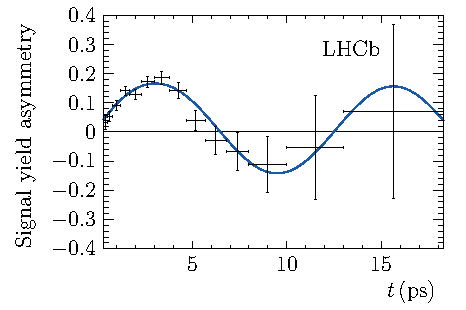
\includegraphics[width=0.6\textwidth]{03CPV/figs/InterferenceCPV.pdf}
	\caption{Time-dependent signal yield asymmetry $\left(N_{\Bzb}-N_{\Bz}\right)/\left(N_{\Bzb}+N_{\Bz}\right)$. The black points represent the used datasample, the blue solid curve is the projection of the signal \PDF.}
	\label{fig:sin2beta}
\end{figure}
